\chapter{\textit{Microkernel}}
A palavra \textit{kernel} é tradicionalmente utilizada para denotar a parte do SO que é essencial e comum a todos os outros \textit{softwares}. A idéia principal da abordagem do \textit{microkernel} é reduzir o tamanho \textit{kernel}, implementando o maior número possível de funções e sub-sistemas fora dele. Esta idéia não é nova, advinda desde 1970. A maioria dos \textit{microkernels} comerciais utilizam a abordagem cliente/servidor. \underline{Exemplos:} Mach, Amoeba e Chorus.

\begin{figure}[H]
  \centering
  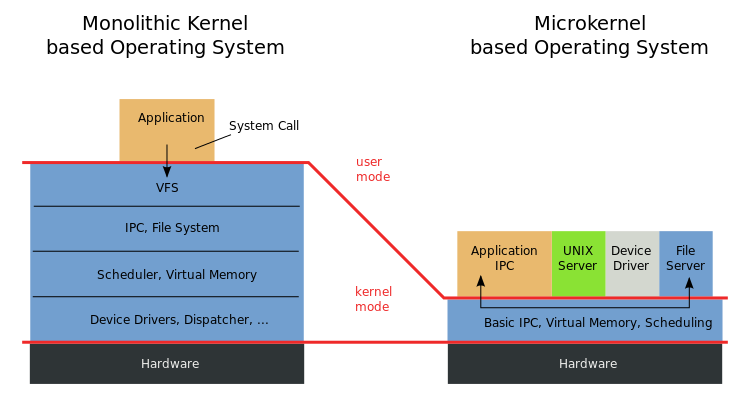
\includegraphics[width=.75\textwidth]{monolithic-2-micro}
  \caption{Comparativo entre a estrutura monolítica e a de \textit{microkernel}}
  \label{fig:monolithic-2-micro}
\end{figure}

\section{Arquitetura}
A interface oferecida garante uma estrutura de sistema mais modular, de forma que o mal-funcionamento de servidores de funções pode ser isolado, como em qualquer outro programa de usuário, protegendo o \textit{kernel} de ser afetado. Além disso, isso permite que diferentes estratégias implementadas por diferentes servidores podem coexistir, garantindo \textbf{maior flexibilidade}.

Entretanto, esta abordagem apresenta a desvantagem inata de possuir \textbf{baixo desempenho}. Tal característica provêm dê:
\begin{itemize}
  \item Aumento do número de tarefas que rodam no modo usuário;
  \item Aumento no número da troca de contextos;
  \item Mecanismo de IPC utilizado entre processos: \textit{send} e \textit{receive}.
\end{itemize}

Com o objetivo de mitigar este problema, a flexibilidade da arquitetura foi sacrificada, para que diversos serviços fossem re-integrados ao \textit{kernel}, evitando as trocas de contexto. Dessa forma, os \textbf{mecanismos que permaneceram no \textit{microkernel} foram}:
\begin{itemize}
  \item Gerência de processos e \textit{threads};
  \item Comunicação de processos;
  \item Proteção e gerência de memória dependente do \textit{hardware};
  \begin{itemize}
    \item Gerênia de memória independente do \textit{hardware} e operações de \textit{page-in} e \textit{page-out} ficam de fora.
  \end{itemize}
\end{itemize}


\subsection{Tratamento de Entrada e Saída}
O espaço de endereçamento é a abstração óbvia para a incorporação de portas de dispositivos. Como o espaço de endereçamento é controlado pelo gerente de memória, o controle de permissão de E/S e os \textit{drivers} de dispositivos \textbf{podem ser implementados fora do \textit{kernel}}.

O \textbf{tratamento de interrupção} neste caso é diferente: o \textit{kernel} recebe a interrupção, transforma-a em mensagem e a envia ao \textit{driver} correspondente, que roda em modo usuário. Desta forma, \textbf{\textit{kernel} não se envolve no tratamento específico de uma interrupção}.

Por sua vez, o \textit{driver} é um processo que acessa diretamente portas de \textit{hardware} em seu espaço de endereçamento e recebe as interrupções via mecanismos de IPC. Caso necessite manipular a memória, pode fazê-lo por meio de gerentes de memória. \underline{Exemplo:} \textit{driver} de vídeo.

\begin{figure}[H]
  \centering
  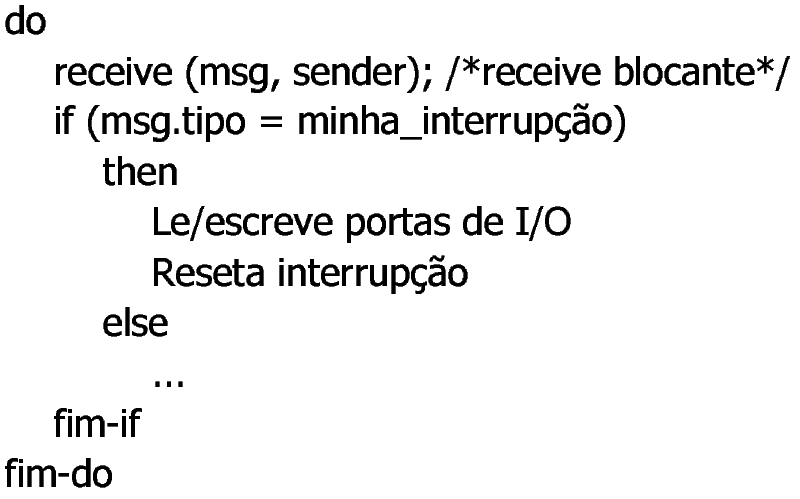
\includegraphics[width=.45\textwidth]{microkernel-driver}
  \caption{Esquema genérico de um \textit{driver} no \textit{microkernel}}
  \label{fig:microkernel-driver}
\end{figure}

\subsection{Identificadores Únicos}
O \textit{microkernel} provê identificadores únicos (\textit{uid}) para recursos como \textit{threads}, tarefas, canais de comunicação, etc.. Logo, se um recurso $S_1$ quer enviar uma mensagem ao recurso $S_2$, ele deve especificar $S_2$ como destino. Para tal, o \textit{microkernel} deve conhecer estes identificadores.

\subsection{Gerentes de Memória}
Um servidor que gerencia o espaço de endereçamento $E0$ será um gerente de memória tradicional, porém fora do \textit{microkernel}. A memória física a ser gerenciada será mapeada para o espaço de endereçamento do servidor.

\subsection{Paginadores}
Os paginadores utilizam as primitivas \textit{grant}, \textit{map} e \textit{flush}, oferecidas pelo \textit{microkernel}. As interfaces entre paginador e cliente, paginador e servidor e paginador e \textit{drivers de dispositivos} são baseadas em IPC e definidas a nível de usuário.









\section{Exemplo: Mach}

\subsection{Modelo de Memória}
No Mach o \textbf{modelo de memória é flexível e independente do \textit{hardware}}. Ele divide a gerência de memória em três partes: \textit{pmap}, modo \textit{kernel} independente de arquitetura e paginador externo.

\subsubsection{\textit{Pmap}}
O Mach admite que cada processador possui sua MMU. Desta forma, o \textit{pmap} é o módulo que irá controlar e acessar a MMU, através de operações em modo protegido. Dessa forma, o \textit{pmap} é dependente da arquitetura de \textit{hardware}.

\subsubsection{\textit{Kernel} Independente de Máquina}
Este módulo trata da parte do processamento do \textit{page fault}, que é independente de máquina. Ele realiza o mapeamento de endereços nas tabelas do sistema e a substituição de páginas.

\subsubsection{Paginador Externo}
Trata da lógica de funcionamento da memória virtual. Portanto, faz:
\begin{itemize}
  \item Gerência da tabela de páginas: cuidando de páginas alocadas e livres, estados das páginas, etc.;

  \item Gerência da atividade de \textit{page-in} e \textit{page-out}: decide quando uma página deve ser carregada em memória (demanda, \textit{prefetching}) e libera o espaço ocupado em memória pela página quando a mesma é escrita em disco.
\end{itemize}

Como o paginador externo roda em modo usuário, várias outras funções podem ser incorporadas a ele.


\subsection{Memória Virtual}
O espaço de endereçamento de um processo é paginado. Este espaço é dividido em unidades esparsas de tamanho variável, chamadas \textbf{regiões}. Cada região que estiver mapeada em memória de um processo é denominada \textbf{objeto de memória}. Eles podem ser arquivos, \textit{pipes}, etc..

Os objetos de memória podem ser gerenciados tanto por paginadores externos como por paginadores \textit{default} do Mach. O objeto de memória é referenciado por uma porta e mensagens são enviadas para solicitar operações sobre o objeto.

Portanto, são definidas primitivas para a memória virtual:
\begin{itemize}
  \item \textbf{\textit{vm\_allocate}:} torna a região de memória utilizável, alocando espaço em uma áreea de memória já mapeada;

  \item \textbf{\textit{vm\_deallocate}:} retira uma região do mapa de memória utilizável;

  \item \textbf{\textit{vm\_map}:} mapeia uma região de memória no espaço de endereçamento do processo. Logo, ela:
  \begin{itemize}
    \item Retorna um ponteiro para o início da região mapeada;

    \item Neste momento, a região é mapeada, porém não é carregada em memória. Assim, o primeiro acesso a esta região ocasionará em um \textit{page fault}.
  \end{itemize}

  \item \textbf{\textit{vm\_copy}:} copia um objeto da memória de uma região para a outra. Como otimização, ele implementa o \textit{copy on write}: o recurso não é efetivamente duplicado, sendo compartilhado até que haja uma escrita em alguma instância;

  \item \textbf{\textit{vm\_inherit}:} determina que regiões serão herdadas na criação de um processo filho;

  \item \textbf{\textit{vm\_read}:} lê de uma região mapeada em outro espaço de endereçamento;

  \item \textbf{\textit{vm\_write}:} escreve uma região mapeada em outro espaço de endereçamento;

\end{itemize}

\subsection{Paginadores Externos}
Objetos de memória são necessariamente paginados, podendo ser \textbf{gerenciados por aplicações de usuário} chamadas gerentes de memória ou paginadores externos. Os gerentes de memória são os responsáveis pelas atividades de \textit{page-in} e \textit{page-out}.

\begin{figure}[H]
  \centering
  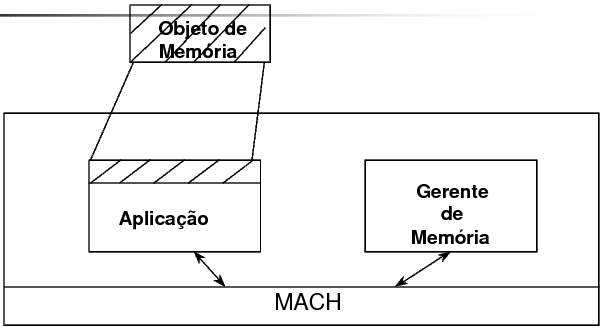
\includegraphics[width=.6\textwidth]{mach-external-pager}
  \caption{Esquema de paginador externo e objeto de memória no espaço da aplicação}
  \label{fig:mach-external-pager}
\end{figure}

\subsubsection{Protocolo entre Gerente e Núcleo}
O gerente de memória interage com o núcleo do \textit{Mach} através de um protocolo assíncrono pré-definido:

\begin{enumerate}
  \item Uma tarefa faz o mapeamento (\textit{vm\_map}) de um objeto de memória sobre o seu espaço de endereçamento. Nesse momento, a tarefa nomeia o gerente de memória como sendo responsável pela gestão do objeto;

  \item O núcleo envia uma mensagem ao gerente de memória (\textit{memory\_object\_init}), dizendo que o objeto que ele gerencia foi mapeado. O gerente faz algumas inicializações e responde ao núcleo com \textit{memory\_object\_ready};

  \item A tarefa referencia o objeto de memória. As referências são feitas por operações básicas de acesso à memória (\textit{LOAD} e \textit{STORE}). Um \textit{page fault} é gerado. O núcleo é ativado e contacta o gerente de memória responsável pelo objeto de memória e pede a página por \textit{memory\_object\_data\_request};

  \item Quando a página estiver disponível, o gerente de memória responde ao \textit{kernel} com \textit{memory\_object\_data\_supply};

  \item A substituição de páginas é decidida pelo núcleo \textit{Mach}. Nesse caso, a página é enviada ao gerente de memória, com um \textit{memory\_object\_data\_return}. O gerente se responsabiliza por armazenar a página;

  \item Se a aplicação deseja referenciar a página de um modo proibido pelos direitos de acesso atuais, um \textit{page fault} de proteção é gerado. O gerente pode também decidir restringir os direitos de acesso à uma página por conta própria.
\end{enumerate}

\begin{figure}[h]
  \centering
  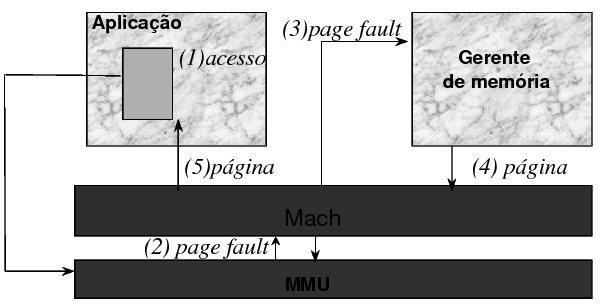
\includegraphics[width=.7\textwidth]{mach-pagination}
  \caption{Protocolo entre gerente e núcleo}
  \label{fig:mach-pagination}
\end{figure}

É importante notar que o usuário pode não querer gerenciar um objeto de memória e deseja que o sistema o faça, uma vez que sendo uma aplicação de usuário, pode conter \textit{bugs}. As páginas que compõe o próprio sistema \textit{Mach} devem ser geradas por alguém. Dado isso, o sistema dispõe de um \textbf{gerente de memória \textit{default}}.

O modelo de memória do \textit{Mach} apresenta grande flexibilidade, porém seu desempenho é baixo. Atualmente, o Unix incorpora parte destas idéias através das primitivas \textit{mmap} e \textit{mprotect}.









\section{Outros Detalhes}

\subsection{Comunicação Remota}
Os \textit{microkernels} foram propostos inicialmente para ambientes distribuídos. O IPC remoto é implementado por servidores que traduzem mensagens locais para protocolos de comunicação externos e vice-versa.





\section{Modelos Alternativos}

\subsection{Ênfase em Portabilidade}
\textbf{\textit{Microkernels} antigos} eram construídos de maneira independente de \textit{hardware}, em cima de uma pequena camada dependente de \textit{hardware}. Esta última tem as seguintes implicações:
\begin{itemize}
  \item Características específicas do \textit{hardware} não podem ser aproveitadas;

  \item A camada de abstração de \textit{hardware} introduz um custo no desempenho.
\end{itemize}

Mesmo com todo este cuidado, em alguns momento, o \textit{microkernel} deve estar consciente das características do \textit{hardware}, que envolvem implementação do espaço de endereçamento do usuário. \underline{Exemplo:} registradores de segmento no Pentium ou a troca de contexto tradicional no i486.

Justamente por esta camada de abstração do \textit{hardware}, o desempenho nestas abordagens acabou por ficar lento.

Arquiteturas diferentes requerem técnicas de otimização específicas que muitas vezes afetam a estrutura global do \textit{microkernel}. Portanto, os \textit{microkernels} mais recentes não são portáveis, sendo a base dependente da arquitetura sobre a qual serão construídos sistemas operacionais portáveis.




\subsection{Domínios de Proteção}
É uma outra estruturação possível além do cliente/servidor, tendo como exemplo as implementações SPACE, Kea, Spring e Pebble. Elas são baseadas em duas abstrações, domínios de proteção e \textit{threads}, onde um programa consiste de: um conjunto de domínios de proteção e uma única \textit{thread}.

O \textbf{domínio de proteção} é composto por um espaço de endereçamento e informações de proteção. Os módulos do sistema operacional são implementados como domínios de proteção. Cada domínio registra seus métodos e o mecanismo de comunicação inter-domínio (IDC) é utilizado para se obter acesso a um método protegido de outro domínio. Existe uma pilha de domínios de proteção que contém as IDCs em andamento.

Como \textbf{vantages} em relação a abordagem cliente/servidor, esta implementação reduz o \textit{overhead} da troca de mensagens e o da troca de contexto entre \textit{threads}. Como \textbf{desvantagem}, ele introduz o \textit{overhead} da pilha de domínio de proteção.






\section{Três Níveis de Proteção}
Outra estruturação possível, baseada nos níveis de proteção da arquitetura Intel x86, que tem 4 níveis de proteção. É implementada pelo \textit{Paladium}.

Em um dado momento, um processo está em um nível de proteção e só pode acessar dados no mesmo nível ou em níveis inferiores, dado que o código só pode ser acessado no mesmo nível de proteção.

Logo, são implementados os \textbf{call gates}. Cada nível de proteção define quais dos seus métodos são acessíveis através de um \textit{call gate}, onde o nível pode ter um número qualquer de \textit{gates}. O \textit{call gate} por sua vez será utilizado para movimentação entre os níveis de proteção.

O espaço de endereçamento de um processo é divido em três níveis: \textit{kernel}, intermediário e usuário.

Cada módulo do SO independe do \textit{hardware} é implementado como um módulo no nível intermediário. Um \textit{call gate} é definido, onde estão incluídos os métodos do módulo (interface). Assim, a comunicação é feita por \textit{call gates}.

Como \textbf{vantagem} em relação ao modelo cliente/servidor, esta implementação reduz o \textit{overhead} da troca de mensagens, troca de contexto entre \textit{threads} e da troca de espaços de endereçamento. Como \textbf{desvantagens}, vemos que esse modelo é dependente do \textit{hardware} dados os níveis de proteção e os módulos do SO não estão protegidos entre si.
